\documentclass[border=10pt]{standalone}
\usepackage{tikz}
\begin{document}
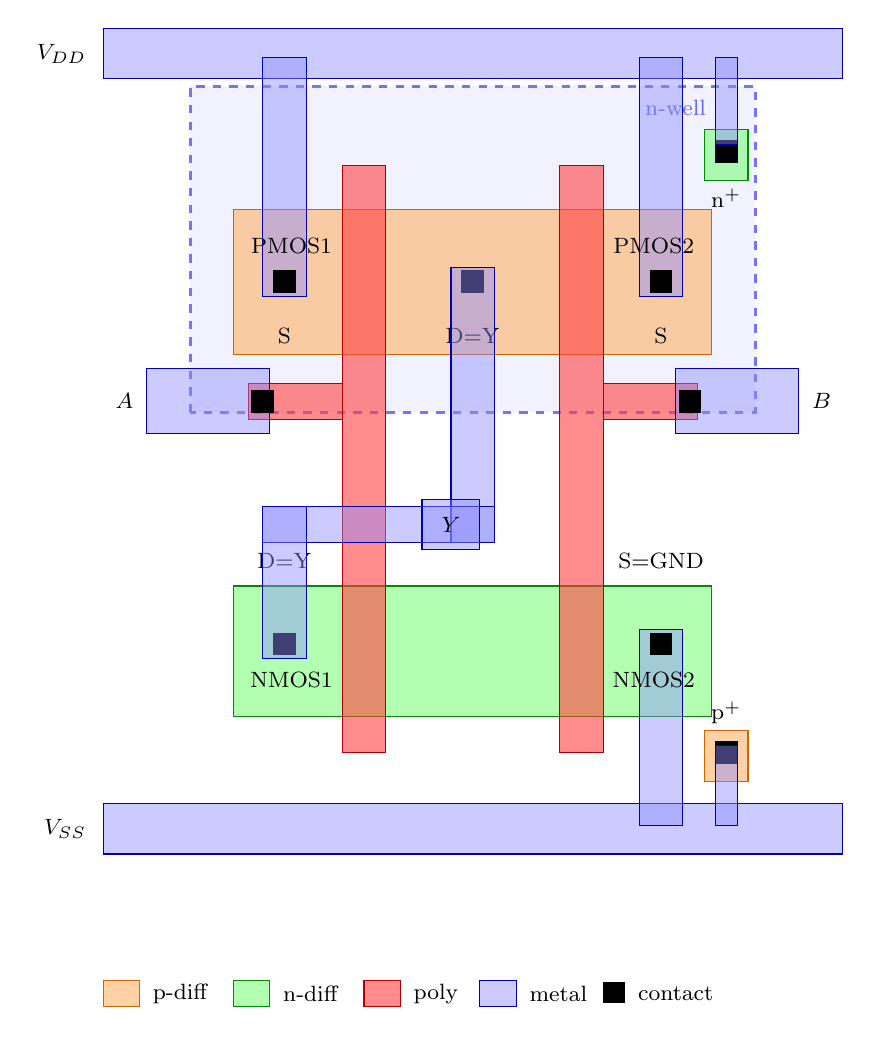
\begin{tikzpicture}[scale=0.92,
  nwell/.style ={draw=blue!55, dashed, line width=1pt, fill=blue!5},
  pdiff/.style ={draw=orange!80!black, fill=orange!65, fill opacity=0.55},
  ndiff/.style ={draw=green!55!black, fill=green!60, fill opacity=0.5},
  poly/.style  ={draw=red!70!black,  fill=red!75,  fill opacity=0.6},
  metal/.style ={draw=blue!70!black, fill=blue!45, fill opacity=0.45},
  cont/.style  ={draw=black, fill=black},
  lbl/.style   ={font=\footnotesize}]

  % ---------------- power rails ----------------
  \fill[metal] (0.4,11.0) rectangle (10.6,11.7);  \node[lbl,left] at (0.3,11.35){$V_{DD}$};
  \fill[metal] (0.4,0.3)  rectangle (10.6,1.0);    \node[lbl,left] at (0.3,0.65){$V_{SS}$};

  % ---------------- n-well around the PMOS pair ----------------
  \fill[nwell] (1.6,6.4) rectangle (9.4,10.9);
  \node[lbl,blue!60] at (8.3,10.6){n-well};

  % ---------------- active areas ----------------
  \fill[pdiff] (2.2,7.2) rectangle (8.8,9.2);   % PMOS (shared p-diffusion)
  \fill[ndiff] (2.2,2.2) rectangle (8.8,4.0);   % NMOS (shared n-diffusion, series)

  % ---------------- two poly gates A (left) and B (right) ----------------
  \fill[poly] (3.7,1.7) rectangle (4.3,9.8);    % gate A
  \fill[poly] (6.7,1.7) rectangle (7.3,9.8);    % gate B
  % gate A input pad (left), tab high in the field gap
  \fill[poly]  (3.7,6.3) rectangle (2.4,6.8);
  \fill[metal] (1.0,6.1) rectangle (2.7,7.0);  \fill[cont] (2.45,6.4) rectangle (2.75,6.7);
  \node[lbl,left] at (0.95,6.55){$A$};
  % gate B input pad (right), tab high in the field gap
  \fill[poly]  (7.3,6.3) rectangle (8.6,6.8);
  \fill[metal] (8.3,6.1) rectangle (10.0,7.0); \fill[cont] (8.35,6.4) rectangle (8.65,6.7);
  \node[lbl,right] at (10.05,6.55){$B$};

  % ---------------- PMOS sources -> VDD (outer ends) ----------------
  \fill[metal] (2.6,8.0) rectangle (3.2,11.3); \fill[cont] (2.75,8.05) rectangle (3.05,8.35);
  \fill[metal] (7.8,8.0) rectangle (8.4,11.3); \fill[cont] (7.95,8.05) rectangle (8.25,8.35);
  \node[lbl] at (2.9,7.45){S}; \node[lbl] at (8.1,7.45){S};
  % PMOS common drain (centre) = Y
  \fill[cont] (5.35,8.05) rectangle (5.65,8.35);
  \node[lbl] at (5.5,7.45){D=Y};

  % ---------------- NMOS series : drain Y (left) , source GND (right) ----------------
  \fill[cont] (2.75,3.05) rectangle (3.05,3.35);   % Y drain (left)
  \node[lbl] at (2.9,4.35){D=Y};
  \fill[metal] (7.8,0.7) rectangle (8.4,3.4); \fill[cont] (7.95,3.05) rectangle (8.25,3.35);
  \node[lbl] at (8.1,4.35){S=GND};

  % ---------------- output Y metal : PMOS centre drain -> NMOS left drain + Y pad ----------------
  \fill[metal] (5.2,4.6) rectangle (5.8,8.4);      % down from PMOS drain
  \fill[metal] (2.6,4.6) rectangle (5.8,5.1);      % across to the left (over field gap)
  \fill[metal] (2.6,3.0) rectangle (3.2,5.1);      % down to NMOS drain
  \fill[metal] (4.8,4.5) rectangle (5.6,5.2);      % central Y pad
  \node[lbl] at (5.2,4.85){$Y$};

  % ---------------- well/substrate taps ----------------
  \fill[ndiff] (8.7,9.6) rectangle (9.3,10.3); \fill[cont] (8.85,9.85) rectangle (9.15,10.15);
  \fill[metal] (8.85,10.1) rectangle (9.15,11.3); \node[lbl] at (9.0,9.35){n$^{+}$};
  \fill[pdiff] (8.7,1.3) rectangle (9.3,2.0); \fill[cont] (8.85,1.55) rectangle (9.15,1.85);
  \fill[metal] (8.85,0.7) rectangle (9.15,1.8); \node[lbl] at (9.0,2.25){p$^{+}$};

  % ---------------- device labels ----------------
  \node[lbl] at (3.0,8.7){PMOS1}; \node[lbl] at (8.0,8.7){PMOS2};
  \node[lbl] at (3.0,2.7){NMOS1}; \node[lbl] at (8.0,2.7){NMOS2};

  % ---------------- legend ----------------
  \begin{scope}[shift={(0,-2.3)}]
    \fill[pdiff](0.4,0.5) rectangle(0.9,0.85); \node[lbl,right] at(0.95,0.67){p-diff};
    \fill[ndiff](2.2,0.5) rectangle(2.7,0.85); \node[lbl,right] at(2.75,0.67){n-diff};
    \fill[poly] (4.0,0.5) rectangle(4.5,0.85); \node[lbl,right] at(4.55,0.67){poly};
    \fill[metal](5.6,0.5) rectangle(6.1,0.85); \node[lbl,right] at(6.15,0.67){metal};
    \fill[cont] (7.3,0.55) rectangle(7.6,0.82); \node[lbl,right] at(7.65,0.67){contact};
  \end{scope}
\end{tikzpicture}
\end{document}
